\documentclass[noamssymb,svgnames]{beamer}
\usecolortheme{beaver}
%\useinnertheme[shadow]{rounded}
\usefonttheme{serif}
\usefonttheme{professionalfonts}

\usepackage[bitstream-charter]{mathdesign} % Use BT Charter font
\usepackage[T1]{fontenc}                   % Use T1 encoding instead of OT1
\usepackage[utf8]{inputenc}                % Use UTF8 input encoding
\usepackage{microtype}                     % Improve typography
\usepackage{booktabs}
\usepackage[binary-units]{siunitx}
\usepackage{tikz}
\usetikzlibrary{shapes.geometric}

\usepackage{hyperref}
\hypersetup{pdfstartview=Fit}

% BEAMER CONFIGURATION ---------------------------------------------------------
\setbeamerfont{block title}{size=\normalsize}
\setbeamerfont{block body}{size=\scriptsize}
\setbeamercolor{block title}{fg=darkred,bg=gray!10!white}
\setbeamercolor*{item}{fg=darkred}

\usepackage[many,minted]{tcolorbox}

% Set ipython options
\setminted[ipythonconsole]{
  mathescape,
  autogobble,
  fontsize=\tiny,
  fontfamily=courier,
  framesep=2mm
}

% -----------------------------------------------------------------------------
\title{Overview of OpenMC}

\institute{
\includegraphics[width=2in]{../images/openmc_logo.png}}

\date{OpenMC Workshop \\ Canadian Nuclear Laboratories \\ March 14--16, 2017}

% -----------------------------------------------------------------------------
\begin{document}

\frame{\titlepage}

% -----------------------------------------------------------------------------
%\begin{frame}{OpenMC}
%  \begin{itemize}
%  \item Open source continuous-energy Monte Carlo particle transport code
%    developed by ANL, MIT, and other contributors
%  \item Currently only neutron transport (photon transport in development)
%  \item Particular focus on HPC, ease of use, methods development
%  \item Input scripts (Python API) generate XML files, HDF5 output files
%  \item Most applications to-date have been reactors / criticality
%  \end{itemize}
%\end{frame}

\begin{frame}{Goals of the OpenMC Project}
  Develop a Monte Carlo particle transport code that:
  \begin{itemize}
  \item Scales on leadership-class supercomputers (100,000+ cores)
  \item Is easy to understand and suitable for methods development
  \item Adopts modern programming paradigms
  \item Is open source, freely available, with permissive licensing
  \item Most of all, is fun to use and has a thriving community!
  \end{itemize}
\end{frame}

\begin{frame}{History of OpenMC}
  \begin{itemize}
  \item Development began in 2011 primarily for two reasons:
    \begin{enumerate}
    \item Parallel scaling in other codes was observed to be quite bad
    \item Export control restrictions made research continuity difficult
    \end{enumerate}
  \item Received green light from DOE/NNSA in early 2012 for open release
  \item Python API added in 2015
  \item Received formal funding from DOE in Sep. 2016 as part of Exascale
    Computing Project
  \item 16 releases so far
  \end{itemize}
\end{frame}

\begin{frame}{Features of OpenMC}
  \begin{columns}[T]
    \column{0.5\textwidth}
    \begin{block}{Current features}
      \begin{itemize}
      \item Fixed source and $k$-eigenvalue calculations
      \item \textbf{Geometry}: CSG with second-order surfaces, repeated geometry units
      \item \textbf{Cross sections}: Continuous-energy or multi-group
      \item \textbf{Physics}: Only neutron transport
      \item \textbf{Tallies}: Flexible general tally system
      \item \textbf{Parallelism}: MPI/OpenMP
      \item \textbf{Input}: XML or Python API-driven
      \item \textbf{Output}: HDF5
      \item Coarse-mesh finite-difference acceleration
      \item Multi-group cross section generation
      \item Nuclear data processing
      \end{itemize}
    \end{block}
    \column{0.5\textwidth}
    \begin{block}{Short-term}
      \begin{itemize}
      \item Depletion
      \item Photon transport
      \item Thermal-hydraulics coupling
      \item Domain decomposition
      \end{itemize}
    \end{block}
    \begin{block}{Medium-term}
      \begin{itemize}
      \item Non-CSG deformable geometry
      \item Transient-capability
      \item Coupling with MOOSE
      \end{itemize}
    \end{block}
  \end{columns}
\end{frame}

\begin{frame}{Parallel Performance}
  \begin{columns}
    \column{0.35\textwidth}
    \begin{center}
      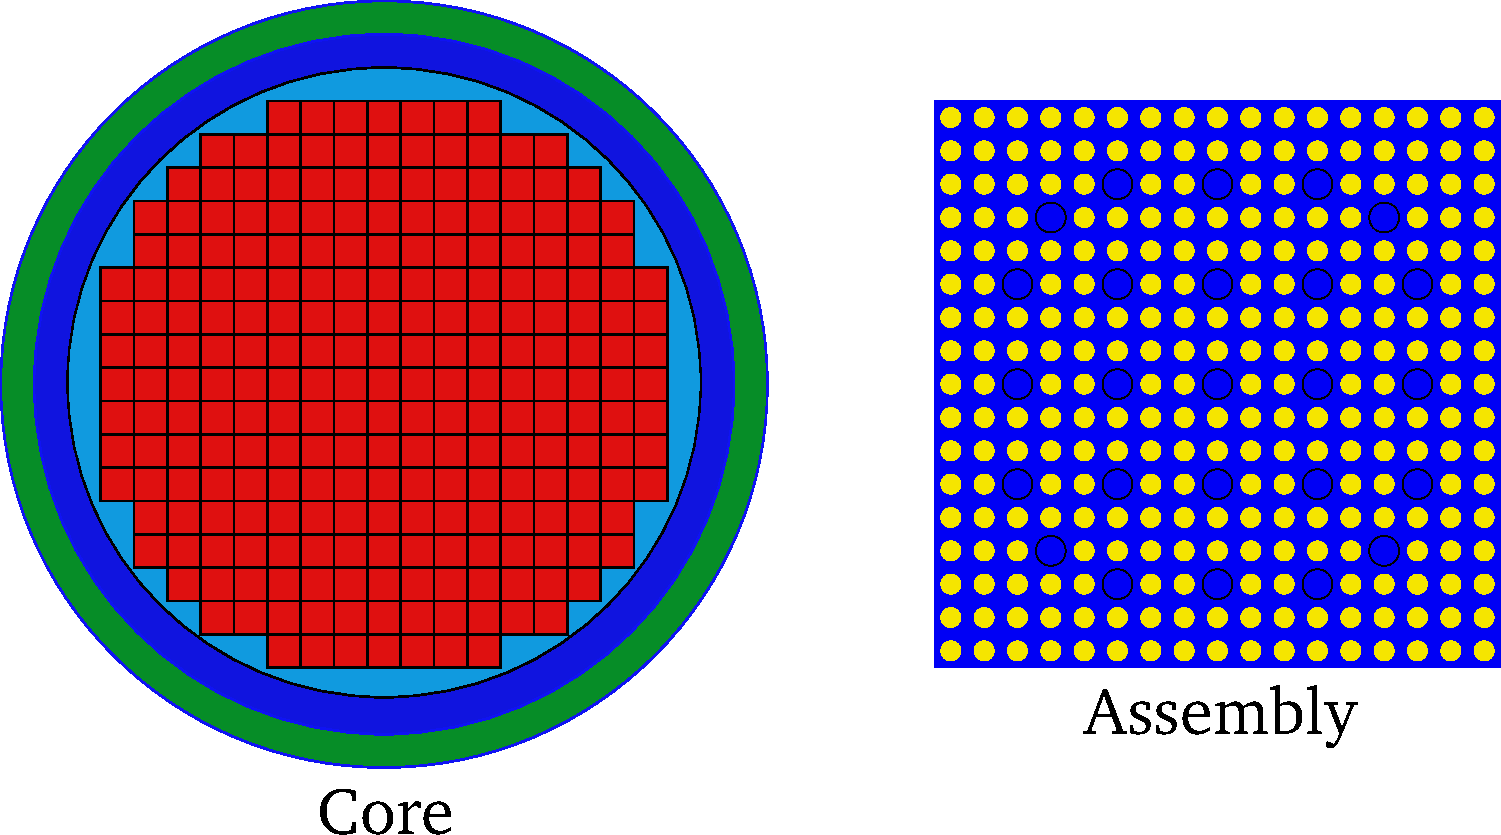
\includegraphics[width=1.7in]{../images/mcperformance.pdf}
    \end{center}
    \footnotesize{
      \begin{itemize}
      \item Mira -- \#5 on TOP 500
      \item 49,152 nodes, 786,432 cores
      \item 4 hw threads/core = 3,145,728 threads
      \end{itemize}
    }
    \column{0.65\textwidth}
    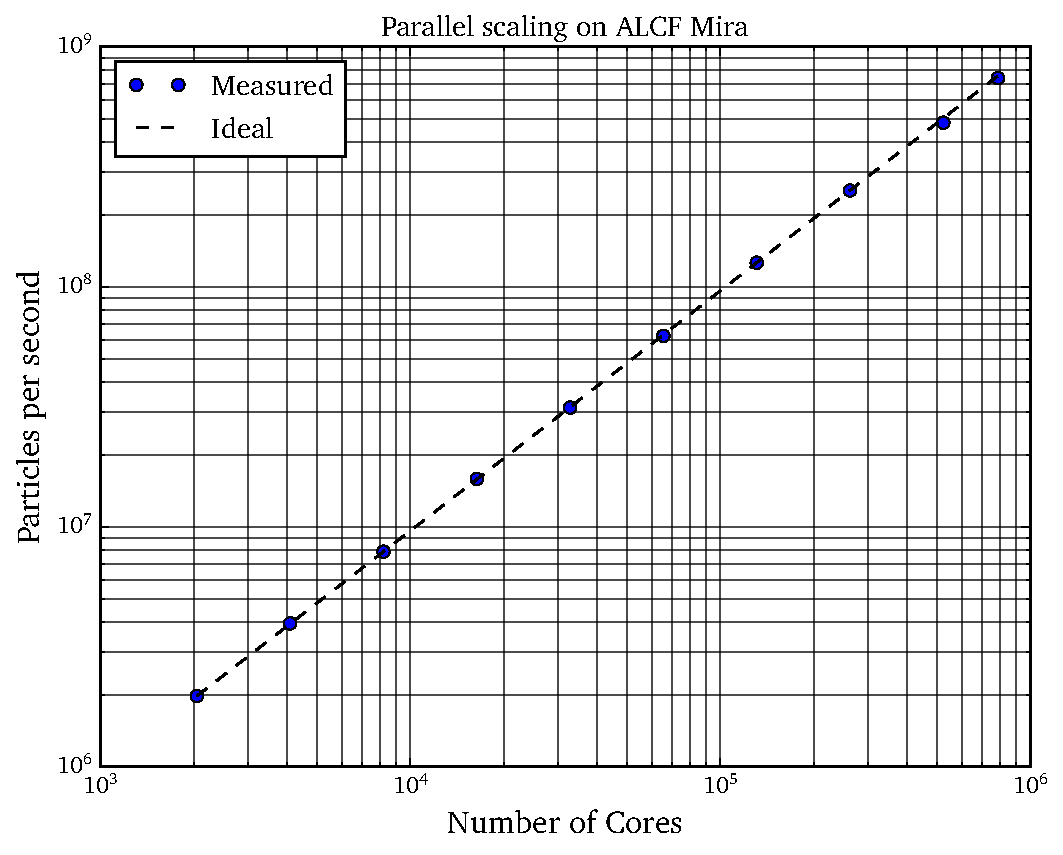
\includegraphics[width=3.0in]{../images/scaling_loglog.pdf}
  \end{columns}
\end{frame}

\begin{frame}{Validation and Verification}
  \begin{itemize}
  \item MCNP Criticality Benchmark Suite
    \begin{itemize}
    \item 119 configurations --- different spectra, materials, enrichment
    \item Models built for all but two
    \end{itemize}
  \end{itemize}
  \centerline{
    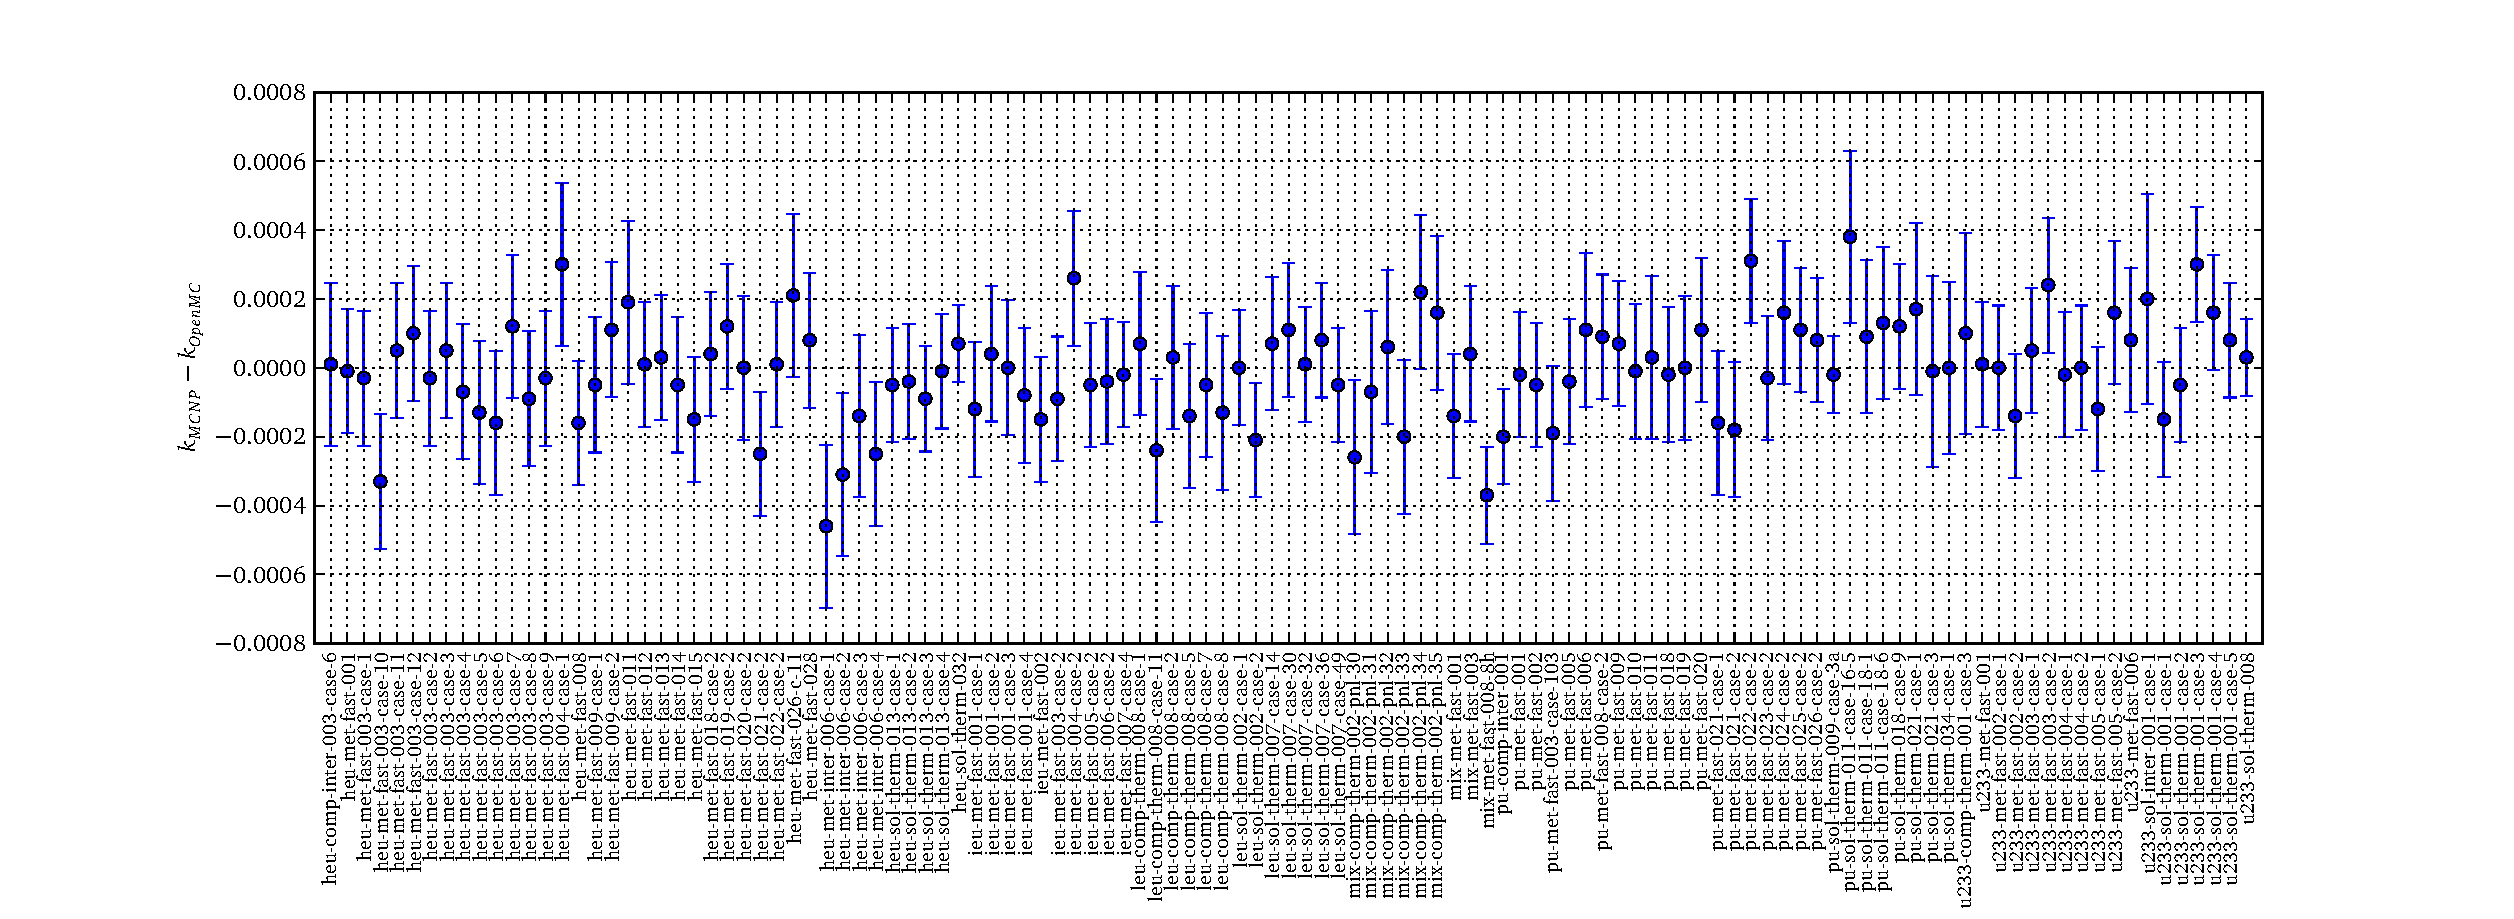
\includegraphics[width=1.35\textwidth]{../images/expanded-suite.pdf}
  }
\end{frame}

\begin{frame}{Example: MIT BEAVRS Benchmark}
  \begin{columns}
    \column{0.5\textwidth}
    \small
    \begin{itemize}
    \item Radial enrichment zoning
    \item Guide tubes/instrument tubes
    \item Burnable absorbers/control rods
    \item Grid spacers, core support
    \item Core baffel, core barrel
    \item Thermal shield pads
    \item Reactor pressure vessel
    \end{itemize}
    \column{0.5\textwidth}
    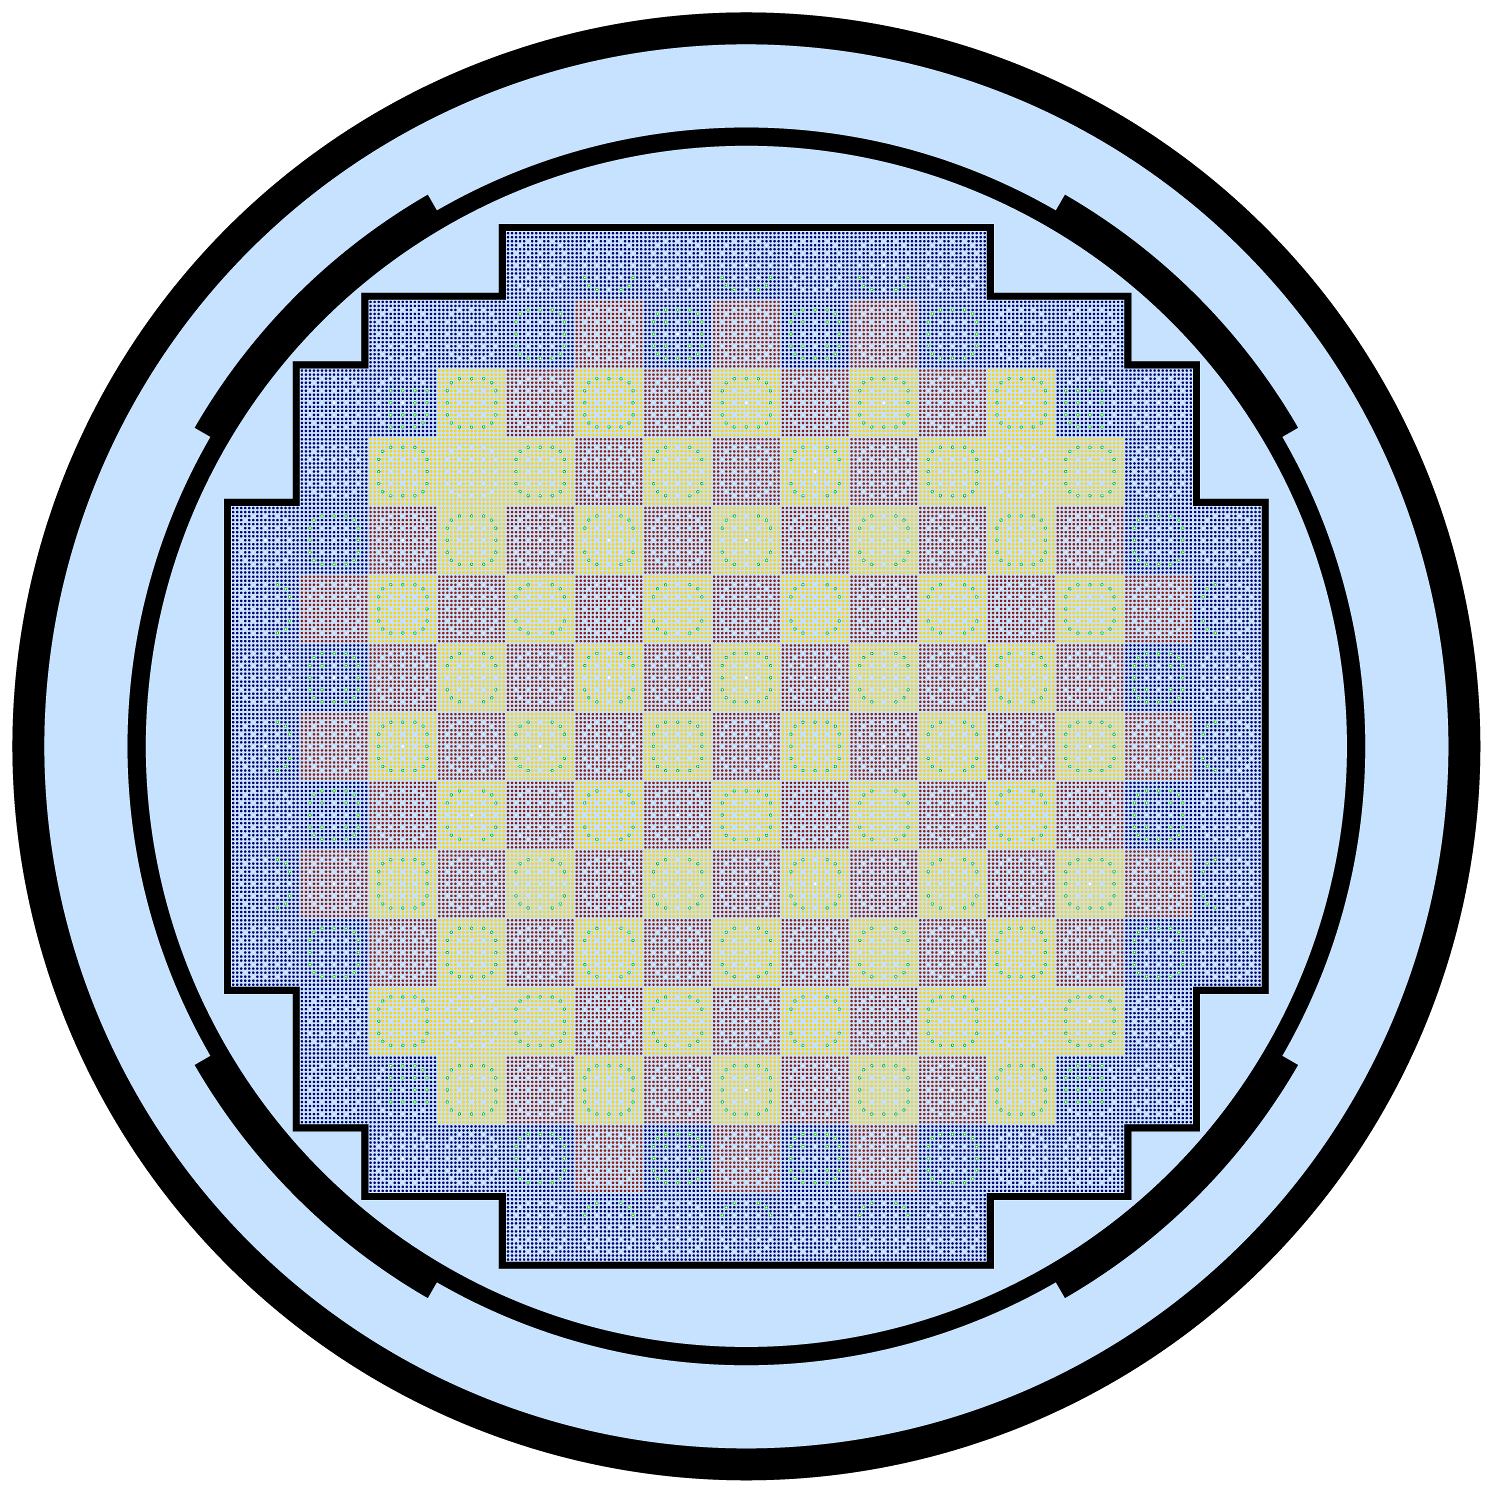
\includegraphics[width=\textwidth]{../images/beavrs_lowerres.png}
  \end{columns}
\end{frame}

\begin{frame}{Example: Advanced Test Reactor}
  \begin{center}
    
\includegraphics[width=0.7\textwidth]{../images/atr.png}
  \end{center}
\end{frame}

\begin{frame}{Software Architecture}
  \begin{itemize}
  \item $\sim$46,000 lines of \textbf{Fortran 2008} code
  \item Relies on \textbf{pugixml} XML parser (C++)
  \item Distributed-memory parallelism via \textbf{MPI}
  \item Shared-memory parallelism via \textbf{OpenMP}
  \item \textbf{CMake} build system for portability
  \item $\sim$45,000 lines of \textbf{Python} API
  \item Version control through \textbf{git}
  \item Code hosting, bug tracking through \textbf{GitHub}
    \begin{itemize}
    \item \url{https://github.com/mit-crpg/openmc}
    \end{itemize}
  \item Automatic documentation generation with \textbf{Sphinx}
    \begin{itemize}
    \item \url{http://openmc.readthedocs.org/en/latest}
    \end{itemize}
  \end{itemize}
\end{frame}

\begin{frame}{XML Input}
  \begin{itemize}
  \item When you run \textbf{openmc} command, it looks for a set of XML files:
    \begin{itemize}
    \item Paramters for the simulation --- \textbf{settings.xml}
    \item Material definitions --- \textbf{materials.xml}
    \item Geometric model, mapping of materials --- \textbf{geometry.xml}
    \item Determine which quantities to score --- \textbf{tallies.xml}
    \item Create geometry plots --- \textbf{plots.xml}
    \end{itemize}
  \item Writing XML files is now considered ``old-school''
  \end{itemize}
\end{frame}

\begin{frame}{Python API Input}
  \begin{itemize}
  \item OpenMC includes a rich Python API that enables programmatic pre- and
    post-processing
  \item To construct input files (and analyze output) you, as the user,
    \emph{must write a Python script} utilizing classes defined by the OpenMC
    API
  \item There are many benefits to using Python API over direct use of XML,
    e.g.,
    \begin{itemize}
    \item All the usual benefits of Python -- variables vs. hard-coded numbers,
      standard library, third-party packages
    \item Run-time type checking
    \item Perturbation or sensitivity studies
    \item Extra features in our API -- data analysis, multi-group cross section
      generation, nuclear data parsers, etc.
    \end{itemize}
  \item \textbf{Caveat:} You need to know Python!
  \end{itemize}
\end{frame}

\begin{frame}{Resources}
  \begin{itemize}
  \item User's Group: \url{openmc-users@googlegroups.com}
  \item Developer's Group: \url{openmc-dev@googlegroups.com}
  \item Documentation: \url{http://openmc.readthedocs.org/en/latest/}
  \end{itemize}
\end{frame}

\end{document}
